
\documentclass{article}



\usepackage{graphicx,comment,framed}
\usepackage{roundbox}
\usepackage{fancybox}
\usepackage{tikz}
\usepackage{color}
\usepackage[hidelinks]{hyperref}
\usepackage{framed}
\usepackage{amsthm,amssymb,amsmath}
%\usepackage[colorlinks,linkcolor=blue,citecolor=blue]{hyperref}
\definecolor{shadecolor}{cmyk}{0,0,0,0}
\usepackage{listings}
\usepackage{xepersian}
\usepackage[noend]{algpseudocode}


%--------------------- page settings ----------------------

\settextfont[Scale=1.1]{XB Niloofar}
\setdigitfont[Scale=1.1]{XB Niloofar}
\defpersianfont\sayeh[Scale=1.1]{XB Niloofar}
\addtolength{\textheight}{3.2cm}
\addtolength{\topmargin}{-22mm}
\addtolength{\textwidth}{3cm}
\addtolength{\oddsidemargin}{-1.5cm}


%------------------------ Environments ------------------------------------

\newtheorem{قضیه}{قضیه}
\newtheorem{لم}{لم}
\newtheorem{مشاهده}{مشاهده}
\newtheorem{تعریف}{تعریف}


%-------------------------- Notations ------------------------------------

\newcommand{\IR}{\ensuremath{\mathbb{R}}} 
\newcommand{\IZ}{\ensuremath{\mathbb{Z}}} 
\newcommand{\IN}{\ensuremath{\mathbb{N}}} 
\newcommand{\IS}{\ensuremath{\mathbb{S}}} 
\newcommand{\IC}{\ensuremath{\mathbb{C}}} 
\newcommand{\IB}{\ensuremath{\mathbb{B}}} 

\newcommand{\bR}{\mathbb{R}}
\newcommand{\cB}{\mathcal{B}}
\newcommand{\cO}{\mathcal{O}}
\newcommand{\cG}{\mathcal{G}}
\newcommand{\rM}{\mathrm{M}}
\newcommand{\rC}{\mathrm{C}}
\newcommand{\rV}{\mathrm{V}}

\newcommand{\lee}{\leqslant}
\newcommand{\gee}{\geqslant}
\newcommand{\ceil}[1]{{\left\lceil{#1}\right\rceil}}
\newcommand{\floor}[1]{{\left\lfloor{#1}\right\rfloor}}
\newcommand{\prob}[1]{{\mbox{\tt Pr}[#1]}}
\newcommand{\set}[1]{{\{ #1 \}}}
\newcommand{\seq}[1]{{\left< #1 \right>}}
\newcommand{\provided}{\,|\,}
\newcommand{\poly}{\mbox{\rm poly}}
\newcommand{\polylog}{\mbox{\rm \scriptsize polylog}\,}
\newcommand{\comb}[2] {\left(\!\!\begin{array}{c}{#1}\\{#2}\end{array}\!\!\right)}




\newcounter{probcnt}
\newcommand{\مسئله}[1]{\stepcounter{probcnt}\bigskip\bigskip{
 	\large \bf مسئله‌ی \arabic{probcnt}$\mbox{\bf{.}}$ \ #1} \bigskip}

\newcommand{\fqed}[1]{\leavevmode\unskip\nobreak\quad\hspace*{\fill}{\ensuremath{#1}}}

\newenvironment{اثبات}
	{\begin{trivlist}\item[\hskip\labelsep{\em اثبات.}]}
	{\fqed{\square}\end{trivlist}}

\newenvironment{حل}
	{\begin{trivlist}\item[\hskip\labelsep{\bf حل.}]}
	{\fqed{\blacktriangleright}\end{trivlist}}

\ifdefined\hidesols
	\newsavebox{\trashcan} % uncomment the following line to hide solutions
	\renewenvironment{حل}{\begin{latin}\begin{lrbox}{\trashcan}}{\end{lrbox}\end{latin}}
\fi


%------------------------- Header -----------------------------

%------------------------- Header -----------------------------

\newcommand{\سربرگ}[3]{
	\parindent=0em
	\begin{shaded}
		
		\rightline{ 
			\makebox[6em][c]{
				
\includegraphics[height=1.6cm]{aut.png}
		}}
		\vspace{-.2em}
		{\scriptsize\bf دانشکده‌ی مهندسی کامپیوتر}
		\hfill {\small
			مدرس: دکتر امیرمزلقانی  \ 
		}\\[-5em]
		\leftline{\hfill\Large\bf 
			کاربرد های جبر خطی
		}\\[.7em]
		\leftline{\hfill\bf 
			نیم‌سال دوم ۹۶-۹۷
		}\\[1.7em]
		\hrule height .12em
		
		\normalsize
		\vspace{1mm} #1
		\hfill \small  #3
		\vspace{1mm} 
		\hrule height .1em
		
		\vspace{-0.5em} 
		\hfill {\sayeh\large #2} \hfill
	\end{shaded}
	\begin{large}

توجه:
\end{large}
\\
\\
\begin{itemize}
\item
این تمرین از مباحث مربوط به فصل5 ،6و7 طراحی شده است که شامل 15سوال اجباری و 4 سوال امتیازی است که نمره سوال های امتیازی فقط به نمرات تمرین شما کمک می کند.
\item 
در برخی سوالات چند قسمتی از شما خواسته شده است به تعدادی از قسمت ها به اختیار پاسخ دهید ،پاسخگویی به بیش از مقدار تعیین شده نمره اضافی ندارد ،از بقیه قسمت ها می توانید برای تمرین بیشتر استفاده کنید.
\item 
در پایان نیز تعدادی سوال برای تمرین بیشتر در نظر گرفته شده است ،که به حل آن ها نمره ای تعلق نمی گیرد صرفا برای تمرین توسط خود شما در نظر گرفته شده است. 
\item 
اگه سوالی داشتین از طریق
\begin{latin}
\href{mailto:aut.la2018@gmail.com}{\[aut.la2018@gmail.com\]}
\end{latin}
 حتما بپرسید.

\item پاسخ های تمرین را در قالب یک فایل به صورت الگوی زیر آپلود کنید.
\begin{latin}
9531000\_steve\_McManaman\_HW4.pdf
\end{latin}
\item \color{red}
مهلت تحویل جمعه  1تیر 1397 ساعت 23:54:59
\end{itemize}

}




%\settextfont{Yas}
\begin{document}
\سربرگ{ فصل اول (معادلات خطی در جبر خطی)}{}{}
\clearpage


\clearpage
\section{سوالات شبیه سازی}

\مسئله

دستگاه معادله زیر را در نظر بگیرید

\begin{latin}
	$x_1$ +$3x_3$ +$x_5$ =−1
	
	 $x_1$ + $x_2$ + $x_3$ +$6x_5$ =1
	 
	  $−3x_1$ −$3x_2$ −$3x_3$ +$x_4$ −$19x_5$ = 6
	  
	   10x1 −4x2 +38x3 +2x4 −12x5 = 0
	\end{latin}
\begin{enumerate}
	\item
	ماتریس افزوده این دستگاه را به نام $A$ایجاد کنید.
	\item 
	با استفاده از اعمال سطری مقدماتی، ماتریس $A$ را به فرم سطری مقدماتی تبدیل کنید.
	\item 
با استفاده از نتیجه قسمت قبل، فرم کاهش یافته سطری ستونی ماتریس $A$  را به دست آورید.
\item 
مجموعه پاسخ این دستگاه را به دست آورید. (مشخص کنید که آیا این دستگاه پایدار است یا خیر و در صورت پایدار بودن اگر متغیر آزاد دارد، متغیر های پایه ای را بر حسب آنها به دست آورید.)
\end{enumerate}

(راهنمایی:
 برای بخش ۲ عملیات سطری مقدماتی در متلب به صورت زیر قابل انجام هستند:
 \begin{itemize}
 	\item 
 	دستور زیر، $-4$ برابر سطر اول ماتریس $A$ را به سطر سوم این ماتریس اضافه می کند
 	\begin{latin}
 		A(3,:)=A(3,:)+(-4)*A(1,:)
 	\end{latin}
  	\item 
 دستور زیر، مقادیر سطر سوم ماتریس $A$ را دو برابر می کند
 \begin{latin}
 	A(3,:)=2*A(3,:)
 \end{latin}
 	\item 
دستور زیر، سطر دوم و سوم ماتریس $A$ را جا به جا می کند
\begin{latin}
	A([2 3],:)=A([3 2],:)
\end{latin}
\end{itemize}
	
)


\clearpage
\مسئله{Gauss-Jordan Elimination}

به فرایند اعمال کردن عملیات سطری مقدماتی $(EROs) $بر روی یک ماتریس برای تبدیل آن به فرم کاهش یافته سطری مقدماتی، حذف گاوس جردن گفته می شود و اگر تنها به فرم سطری مقدماتی بسنده کنیم به آن حذف گاوس گفته می شود.
در این تمرین، شما باید یک تابع بنویسید که با گرفتن یک ماتریس به عنوان ورودی و با اعمال عملیات سطری مقدماتی بر روی آن، فرم کاهش یافته سطری مقدماتی آن و تعداد عملیات سطری مقدماتی انجام شده به این منظور را برگرداند.

جزیات این تابع که آن را $ MyRREF$ می نامیم به صورت شبه کد در ادامه آمده است. فرض کنید ماتریس ورودی $A$، دارای ابعداد $m \times n$ باشد.
در این شبه کد، نام تابع های $MATLAB$ را که به این منظور می توانید استفاده کنید به رنگ قرمز و کامنت ها را به رنگ آبی مشخص کرده ایم.
همان طور که در $MATLAB$  نیز استفاده می شود،  
$A(i,j)$
  بیانگر درایه i,j ام ماتریس $A$ می باشد و 
$A(i,:)$
    بیانگر سطر i ام ماتریس $A$ است. در این شبه کد عملیات سطری مقدماتی بر روی خود ماتریس ورودی  $A$ اعمال می شوند، لذا در نهایت ماتریس کاهش یافته سطری مقدماتی آن در خود $A$ قرار می گیرد و $n_e$ تعداد عملیات سطری مقدماتی انجام شده را مشخص می کند.

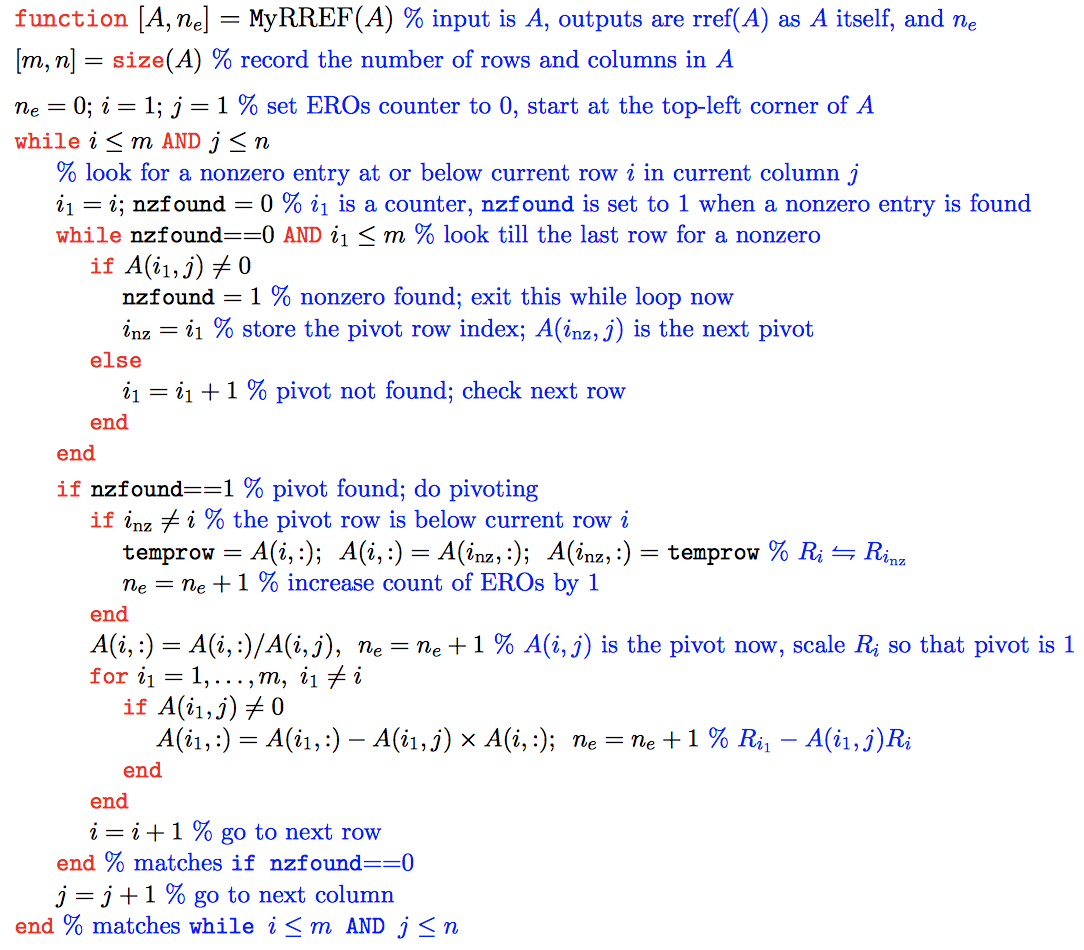
\includegraphics[scale=0.8]{code}
در پیاده سازی استاندارد این تابع، تفاوت های محدودی وجود دارد. برای مثال بزرگ ترین عدد در یک ستون به عنوان pivot استفاده می شود در حالی که در شبه کد فوق، اول عدد غیر صفر انتخاب می گردد.
\clearpage
\begin{enumerate}
	\item 
	این تابع را همانند شبه کد بیان شد پیاده سازی کنید.  همان طور که بیان شد این تابع باید یک ماتریس ورودی A را گرفته و کاهش یافته سطری مقدماتی آن و تعداد عملیات سطری مقدماتی استفاده شده را باز گرداند.
	
	شما می توانید برای اطمینان از درستی تابع خود، خروجی آن را با خروجی تابع آماده متلب به نام rref مقایسه کنید. یک روش برای انجام این مقایسه به صورت زیر است:
\begin{latin}

	[A1, n1] = MyRREF(A);  A2 = rref(A); 

normdiff = norm(A1 − A2);  

\end{latin}
	
	
	خروجی تابع norm یک ماتریس که تمام درایه های آن صفر باشد، صفر خواهد بود. بنابراین اگر خروجی شما برابر خروجی rref باشد، حاصل A1-A2 صفر خواهد شد و در نتیجه norm آن هم صفر است. ولی اگر تفاوت اندکی  بین $A1$  و $A2$ وجود داشته باشد، normdiff یک عدد کوچک غیر صفر خواهد بود و اگر مقدار بزرگی را شود احتمالا یه جای کار اشتباه کرده اید!
	
	\item
	 بررسی کنید که با تغییر تعداد سطر ها و ستون های ماتریس ورودی،‌ تعداد عملیات لازم برای تبدیل به فرم کاهش یافته سطری مقدماتی چه تغییری می کند. به طور خاص برای حالت های زیر تعداد عملیات لازم را به دست آورید. در هر حالت ماتریس ورودی خود را با استفاده از اعداد رندم و از طریق دستور
\begin{latin}
	A = round(1000*rand(m,n))
\end{latin}
	  در متلب تولید کنید.
	 \begin{enumerate}
	 	\item 
	 تعداد سطر ها (m) را ثابت و برابر ۱۰۰ در نظر بگیرید و تابع خود را بر روی ماتریس هایی با تعداد ستون n = 50, 75 , 100, 200, 400, 600, 800,  1000 اجرا کنید. در هر حالت، تعداد عملیات انجام شده و مقدار normdiff را یادداشت کنید و در یک جدول با ستون های n و تعداد عملیات لازم و normdiff نشان دهید.
	 	\item 
	 	تعداد ستون ها (n) را ثابت و برابر ۱۰۰ در نظر بگیرید و تابع خود را بر روی ماتریس هایی با تعداد سطر m = 50, 75 , 100, 200, 400, 600, 800,  1000 اجرا کنید. در هر حالت، تعداد عملیات انجام شده و مقدار normdiff را یادداشت کنید و در یک جدول با ستون های n و تعداد عملیات لازم و normdiff نشان دهید.
	 \end{enumerate}
	
	
	\item 
	 با توجه به مشاهدات انجام شده به سوالات زیر پاسخ دهید:
		 \begin{enumerate}
		 	\item 
		 	تعداد عملیات لازم، هنگامی که تعداد سطر ها ثابت است و تعداد ستون ها تغییر میکند چگونه تغییر میکند؟
		 	\item 
		 	‌ تعداد عملیات لازم، هنگامی که تعداد ستون ها ثابت است و تعداد سطر ها تغییر میکند چگونه تغییر میکند؟
		 	\item 
		 	‌ مقدار normdiff، هنگامی که تعداد سطر ها ثابت است و تعداد ستون ها تغییر میکند چگونه تغییر میکند؟
		 	\item 
		 	‌ مقدار normdiff، هنگامی که تعداد ستون ها ثابت است و تعداد سطر ها تغییر میکند چگونه تغییر میکند؟
		 	 \end{enumerate}
	

\end{enumerate}

\end{document}